\documentclass[11pt]{article}
\usepackage{geometry}                % See geometry.pdf to learn the layout options. There are lots.
\geometry{letterpaper}                   % ... or a4paper or a5paper or ... 
%\geometry{landscape}                % Activate for for rotated page geometry
%\usepackage[parfill]{parskip}    % Activate to begin paragraphs with an empty line rather than an indent
\usepackage{graphicx}
\usepackage{amssymb}
\usepackage{epstopdf}
\DeclareGraphicsRule{.tif}{png}{.png}{`convert #1 `dirname #1`/`basename #1 .tif`.png}

\title{LaTeX Practice}
\author{David Diez}
\date{April 23, 2009}                                           % Activate to display a given date or no date

\begin{document}
\maketitle
%\section{}
%\subsection{}
1) 
\begin{center}
\begin{tabular}{l rrr}
\hline
	& $\bar{x}$ & $\hat{\sigma}$ & $n$ \\
\hline
$S_1$ & 6.5	&	1.3			& 17 \\
$S_2$ & 12.2	&	1.4			& 25 \\
\hline
\end{tabular}
\end{center}

2) As shown in Figure~\ref{lower82}, the $82^{nd}$ percentile of the normal distribution is above the mean. Is this true for every distribution?
\begin{figure}[htbp]
   \centering
   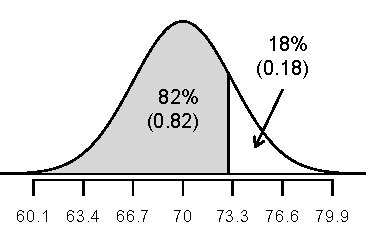
\includegraphics[height=0.8in]{normalPlots/lower82/lower82}
   \caption{The $82^{nd}$ percentile of the normal plot.}
   \label{lower82}
\end{figure}

3)
\begin{eqnarray*}
\sum_{i=0}^n p^{i} = \frac{1-p^{n-1}}{1-p}
\end{eqnarray*}

\end{document}  